\documentclass{article}

\usepackage{shyne}

% document format
\topmargin 0in
\oddsidemargin 0in
\evensidemargin 0in
\headheight 0in
\headsep 0in
\topskip 0in
\textheight 9in
\textwidth 6.5in
\linespread{1.3}

\begin{document}

\begin{flushleft}
\section*{Group Work - Chapter 5}
\paragraph{1} A small town does a census of pet ownership. They find the following distribution of number of dog per household\ldots\\
{\centering
\begin{tabular}{c | c}
Number of dogs & Probability\\
\hline
0 & 0.394\\
1 & 0.342\\
2 & 0.16\\
3 & 0.067\\
4 & 0.036\\
5 & 0.001\\
\end{tabular} \par}
\begin{enumalpha}
\item Is this a probability distribution? What is the expected number of dogs per household? What is the standard deviation? What is the variance?\\
\medskip
\bt{The probabilities add to 1, so this is a probability distribution.}\\
\medskip
{\centering
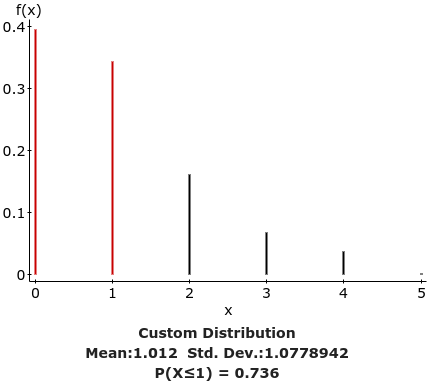
\includegraphics[width=4in]{images/grp05_Q1_a}
\par}
\bt{From StatCrunch, the expected number of dogs in a household, i.e. the mean, is 1.012. Also from StatCrunch, the standard deviation is 1.078. Variance is standard deviation squared. So, variance $\bv{= (1.078)^2 = 1.162}$.}


\vspace{0.25in}
\item What is the probability of a household having at most one dog? Is this unusual? What is the probability of having four or more dogs? Is this unusual?\\
\medskip
$\bv{P(X \le 1) = P(X =0 \btext{ or } X = 1) = P(X=0) + P(X=1) = 0.394 + 0.342 = 0.736}$\\
$\bv{0.736 > 0.05}$ \bt{, so having at most 1 dog is not unusual.}\\
$\bv{P(X \ge 4) = P(X =4 \btext{ or } X = 5) = P(X=4) + P(X=5) = 0.036 + 0.001 = 0.037} $
$\bv{0.037 < 0.05}$ \bt{, so having 4 or more dogs is unusual.}\\
\end{enumalpha}



\newpage
\paragraph{2} The best player on the Metro State basketball team successfully makes 85\% of her free throws. During a typical game she attempts 15 free throws. (If she attempts a different number of free throws, it is not a typical game.)
\begin{enumalpha}
\item Is the number of free throws she makes in a typical game a proper binomial random variable? What are the values of $n$, $p$ and $q$?\\
\medskip
\begin{itemize}
\item \bt{Fixed number of trials (We are only considering typical games where number attempted free throws is 15)}
\item \bt{Two possible outcames (made or not made)}
\item \bt{Each attempt is independent (presumably)}
\item \bt{Each attempt has the same probability (presumably)}
\end{itemize}
\bt{All requirements have been met for a binomial random variable.}\\
\medskip
$\bv{n= 15, \qquad p = 0.85, \qquad q = 1-p = 0.15}$
\vspace{0.25in}

\item What is the expected number of free throws made per game? What is the standard deviation?\\
\medskip
\bt{Expected number of free throws in a game: }$\bv{\E(X) = \mu = np = 15(0.85) = 12.75}$\\
\bt{Standard deviation: }$\bv{\sigma = \sqrt{npq} = \sqrt{(15)(0.85)(0.15)} = 1.383}$

\vspace{.25in}
\item What is the probability she makes all her free throws in a typical game? Is that unusual? What is the probability she makes at least 12 free throws? Less than 12?\\
\medskip
$\bv{P(X=15) = 0.087 > 0.05.}$\bt{ Not unusual.}\\
\medskip
$\bv{P(X \ge 12 ) = 0.823}$ \\
\medskip
$\bv{P(X < 12 ) = 0.177}$\\

\vspace{.25in}

\item What are unusual numbers of free throws made per game?\\
\medskip
$\bv{\mu + 2 \sigma = 12.75 + 2 \times 1.383 = 15.516}$\\
\bt{16 would be an unusually high number of free throws to make, but since the highest possible is 15 there is no unusually high number.}\\
\medskip
$\bv{ \mu - 2 \sigma = 12.75 - 2 \times 1.383 = 9.984}$\\
\bt{9 (or less) free throws made in a game is an unusually low number.}
\end{enumalpha}

\newpage
\paragraph{3} Our taco restaurant, which is open 12 hours a day, get an average of 720 customers a day. For staffing purposes, they are interested in understanding how many customers they might get between 1 and 2 PM. They want to use a Poisson random variable of customers per hour.
\begin{enumalpha}
\item What is the rate of customers per hour ($\lambda$)? If $X \sim Pois(\lambda)$ is the random variable to be used, what is the expected value of $X$? What is the standard deviation?\\
\medskip
\bt{720 customers per 12 hours = 60 customers per hour = $\bv \lambda$}\\
\medskip
$\bv{\E(X) = \mu = \lambda = 60}$\\
\medskip
\bt{Standard deviation }$\bv{= \sigma = \sqrt{\lambda} = \sqrt{60} = 7.746}$

\vspace{0.25in}

\item What is the probability that the restaurant will get 70 or more customers in an hour? What is the probability they will get less than 55? \\
\medskip
$\bv{P(X \ge 70) = 0.112}$\\
\medskip
$\bv{P(X < 55) = 0.242}$\\

\vspace{0.25in}

\item What are unusually high or low numbers of customers per hour?\\
\medskip
$\bv{\mu + 2 \sigma = 60 + 2 \times 7.746 = 75.492}$\\
$\bv{\mu - 2 \sigma = 60 - 2 \times 7.746 = 44.508}$\\
\medskip
\bt{44 (or less) and 76 (or more) are unusual numbers of customers per hour.}

\vspace{0.25in}
\item What is wrong with using this method to predict customers during the hour between 1 and 2 pm?\\
\medskip
\bt{A Poisson distribution assumes that the events are uniformly distributed. However, that is unlikely to be the case in a restaurant. Customers will likely come at higher rates at some times (lunch and dinner) and lower rates at others. Thus, the estimate of 60 customers per hour is likely not accurate for 1 - 2 pm.}

\end{enumalpha}



\end{flushleft}
\end{document}